

\tikzset{every picture/.style={line width=0.75pt}} %set default line width to 0.75pt        

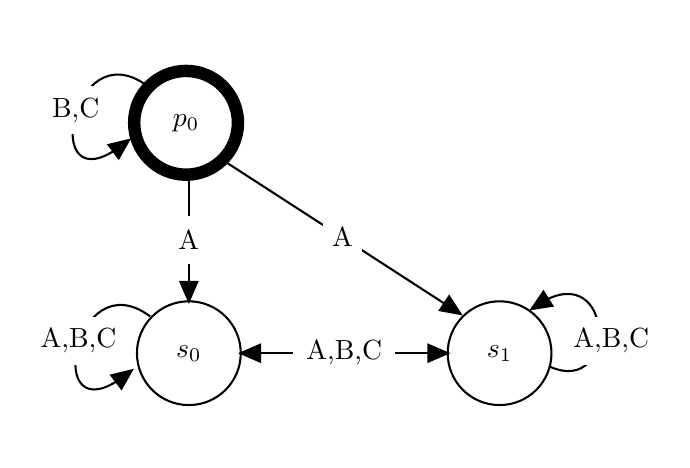
\begin{tikzpicture}[x=0.75pt,y=0.75pt,yscale=-1,xscale=1]
%uncomment if require: \path (0,300); %set diagram left start at 0, and has height of 300

%Shape: Circle [id:dp8938158972072578] 
\draw  [line width=0.75]  (105.29,143) .. controls (105.29,129.19) and (116.48,118) .. (130.29,118) .. controls (144.09,118) and (155.29,129.19) .. (155.29,143) .. controls (155.29,156.81) and (144.09,168) .. (130.29,168) .. controls (116.48,168) and (105.29,156.81) .. (105.29,143) -- cycle ;
%Shape: Circle [id:dp19780391712041556] 
\draw   (255,143) .. controls (255,129.19) and (266.19,118) .. (280,118) .. controls (293.81,118) and (305,129.19) .. (305,143) .. controls (305,156.81) and (293.81,168) .. (280,168) .. controls (266.19,168) and (255,156.81) .. (255,143) -- cycle ;
%Straight Lines [id:da018251469869151382] 
\draw    (155.29,143) -- (255,143) ;


%Shape: Triangle [id:dp4725710951486233] 
\draw  [fill={rgb, 255:red, 0; green, 0; blue, 0 }  ,fill opacity=1 ] (102.8,151.28) -- (97.82,160.08) -- (92.97,153.67) -- cycle ;
%Shape: Triangle [id:dp08394946096129607] 
\draw  [fill={rgb, 255:red, 0; green, 0; blue, 0 }  ,fill opacity=1 ] (255,143) -- (245.72,147.02) -- (245.72,138.98) -- cycle ;
%Shape: Triangle [id:dp12888926826248426] 
\draw  [fill={rgb, 255:red, 0; green, 0; blue, 0 }  ,fill opacity=1 ] (155.29,143) -- (164.56,138.98) -- (164.56,147.02) -- cycle ;
%Shape: Triangle [id:dp7536519811814515] 
\draw  [fill={rgb, 255:red, 0; green, 0; blue, 0 }  ,fill opacity=1 ] (295.43,121.72) -- (301.13,113.37) -- (305.42,120.17) -- cycle ;
%Curve Lines [id:da0862450190271058] 
\draw    (111.62,125.27) .. controls (74.82,97.67) and (59.1,184.08) .. (99.1,154.08) ;


%Curve Lines [id:da8507870813478686] 
\draw    (295.43,121.72) .. controls (335.43,91.72) and (338.63,165.32) .. (303.83,149.32) ;


%Shape: Circle [id:dp06782137726568571] 
\draw  [line width=4.5]  (103.95,32) .. controls (103.95,18.19) and (115.15,7) .. (128.95,7) .. controls (142.76,7) and (153.95,18.19) .. (153.95,32) .. controls (153.95,45.81) and (142.76,57) .. (128.95,57) .. controls (115.15,57) and (103.95,45.81) .. (103.95,32) -- cycle ;
%Shape: Triangle [id:dp8413979641210945] 
\draw  [fill={rgb, 255:red, 0; green, 0; blue, 0 }  ,fill opacity=1 ] (101.46,40.28) -- (96.49,49.08) -- (91.64,42.67) -- cycle ;
%Shape: Triangle [id:dp7368099608094223] 
\draw  [fill={rgb, 255:red, 0; green, 0; blue, 0 }  ,fill opacity=1 ] (261.18,124.1) -- (251.23,122.29) -- (255.69,115.61) -- cycle ;
%Curve Lines [id:da6315070066186073] 
\draw    (110.29,14.27) .. controls (73.49,-13.33) and (57.76,73.08) .. (97.76,43.08) ;


%Straight Lines [id:da7382395640533164] 
\draw    (130.29,59) -- (130.29,118) ;


%Straight Lines [id:da3690444677581517] 
\draw    (147.37,50.44) -- (261.18,124.1) ;


%Shape: Triangle [id:dp417855807516911] 
\draw  [fill={rgb, 255:red, 0; green, 0; blue, 0 }  ,fill opacity=1 ] (130.29,118) -- (126.27,108.72) -- (134.3,108.72) -- cycle ;

% Text Node
\draw (130.29,143) node  [align=left] {$s_0$};
% Text Node
\draw (280,143) node  [align=left] {$s_1$};
% Text Node
\draw  [color={rgb, 255:red, 255; green, 255; blue, 255 }  ,draw opacity=1 ][fill={rgb, 255:red, 255; green, 255; blue, 255 }  ,fill opacity=1 ]  (181.14,132) -- (229.14,132) -- (229.14,154) -- (181.14,154) -- cycle  ;
\draw (205.14,143) node  [align=left] {A,B,C};
% Text Node
\draw  [color={rgb, 255:red, 255; green, 255; blue, 255 }  ,draw opacity=1 ][fill={rgb, 255:red, 255; green, 255; blue, 255 }  ,fill opacity=1 ]  (53.14,126) -- (101.14,126) -- (101.14,148) -- (53.14,148) -- cycle  ;
\draw (77.14,137) node  [align=left] {A,B,C};
% Text Node
\draw  [color={rgb, 255:red, 255; green, 255; blue, 255 }  ,draw opacity=1 ][fill={rgb, 255:red, 255; green, 255; blue, 255 }  ,fill opacity=1 ]  (309.81,126) -- (357.81,126) -- (357.81,148) -- (309.81,148) -- cycle  ;
\draw (333.81,137) node  [align=left] {A,B,C};
% Text Node
\draw (128.95,32) node  [align=left] {$p_0$};
% Text Node
\draw  [color={rgb, 255:red, 255; green, 255; blue, 255 }  ,draw opacity=1 ][fill={rgb, 255:red, 255; green, 255; blue, 255 }  ,fill opacity=1 ]  (59.31,15) -- (92.31,15) -- (92.31,37) -- (59.31,37) -- cycle  ;
\draw (75.81,26) node  [align=left] {B,C};
% Text Node
\draw  [color={rgb, 255:red, 255; green, 255; blue, 255 }  ,draw opacity=1 ][fill={rgb, 255:red, 255; green, 255; blue, 255 }  ,fill opacity=1 ]  (121.29,77.5) -- (139.29,77.5) -- (139.29,99.5) -- (121.29,99.5) -- cycle  ;
\draw (130.29,88.5) node  [align=left] {A};
% Text Node
\draw  [color={rgb, 255:red, 255; green, 255; blue, 255 }  ,draw opacity=1 ][fill={rgb, 255:red, 255; green, 255; blue, 255 }  ,fill opacity=1 ]  (195.27,76.27) -- (213.27,76.27) -- (213.27,98.27) -- (195.27,98.27) -- cycle  ;
\draw (204.27,87.27) node  [align=left] {A};


\end{tikzpicture}
